\documentclass{article}
\usepackage[utf8]{inputenc}
\usepackage{amsmath}
\usepackage{amssymb}
\usepackage{graphicx}


\begin{document}
\section*{Banded matrix}
In this problem we consider for $n \in \mathbb{N}$ the following matrix with $a_{i}, b_{i} \in \mathbb{R}$.
\begin{equation*}
\mathbf{A} :=
    \begin{bmatrix}
    2 & a_{1} & 0 & \dots & \dots & \dots & 0 \\
    0 & 2 & a_{2} & 0 & \dots & \dots & 0 \\
    b_{1} & 0 & \ddots & \ddots & \ddots & & \vdots \\
    0 & b_{2} & \ddots & \ddots & \ddots & \ddots & \vdots \\
    \vdots & 0 & \ddots & \ddots & \ddots & \ddots & 0\\
    \vdots & \vdots & \ddots & \ddots & \ddots & \ddots & a_{n-1} \\
    0  & 0 & \dots & 0 & b_{n-2} & 0 & 2
    \end{bmatrix} \in \mathbb{R}^{n,n}
\end{equation*}
This matrix is an instance of a \textbf{banded matrix}.
\subsection*{2-6.a} We are tasked with implementing an efficient function to compute the result $\mathbf{y}$ of the matrix multiplication $\mathbf{y} = \mathbf{A}\mathbf{x}$. Let us illustrate this matrix-vector multiplication using an example.
\begin{equation*}
    \begin{bmatrix}
    2 & a_{1} & 0 & 0 & 0 & 0& 0 \\
    0 & 2 & a_{2} & 0 & 0& 0 & 0 \\
    b_{1} & 0 & 2 & a_{3} & 0 & 0& 0 \\
    0 & b_{2} & 0& 2& a_{4} & 0& 0\\
    0 & 0 &b_{3} & 0 & 2 & a_{5} & 0\\
    0 & 0 & 0 & b_{4} & 0 & 2 & a_{6} \\
    0  & 0 & 0 & 0 & b_{5} & 0 & 2
    \end{bmatrix}
    \begin{bmatrix}
        x_{1} \\ x_{2} \\ x_{3} \\ x_{4} \\ x_{5} \\ x_{6} \\ x_{7}
    \end{bmatrix} =
    \begin{bmatrix}
        2x_{1} + a_{1}x_{2} \\
        2x_{2} + a_{2}x_{3} \\
        b_{1}x_{1} + 2x_{3} + a_{3}x_{4} \\
        b_{2}x_{2} + 2x_{4} + a_{4}x_{5} \\
        b_{3}x_{3} + 2x_{5} + a_{5}x_{6} \\
        b_{4}x_{4} + 2x_{6} + a_{6}x_{7} \\
        b_{5}x_{5} + 2x_{7}
    \end{bmatrix} = \begin{bmatrix}
        y_{1} \\ y_{2}  \\ y_{3} \\ y_{4} \\ y_{5} \\ y_{6} \\ y_{7}
    \end{bmatrix}
\end{equation*}
We can also write this as
\begin{equation*}
    y_{i} = 
    \begin{cases}
    2x_{i} + a_{i}x_{i +1} \quad &\text{if } i = 1,2 \, , \\
    b_{i - 2}x_{i - 2} + 2x_{i} + a_{i}x_{i+1} &\text{if } 2 < i < n  \, , \\
    b_{i-2}x_{i-2} + 2x_{i} &\text{else.}
    \end{cases}
\end{equation*}
We can also see that we can split this sum into three parts
\begin{equation*}
    \begin{bmatrix}
        y_{1} \\ y_{2}  \\ y_{3} \\ y_{4} \\ y_{5} \\ y_{6} \\ y_{7}
    \end{bmatrix} = \begin{bmatrix}
        2x_{1} + a_{1}x_{2} \\
        2x_{2} + a_{2}x_{3} \\
        b_{1}x_{1} + 2x_{3} + a_{3}x_{4} \\
        b_{2}x_{2} + 2x_{4} + a_{4}x_{5} \\
        b_{3}x_{3} + 2x_{5} + a_{5}x_{6} \\
        b_{4}x_{4} + 2x_{6} + a_{6}x_{7} \\
        b_{5}x_{5} + 2x_{7}
    \end{bmatrix}
    = \begin{bmatrix}
        0 \\ 0 \\ b_{1}x_{1} \\
        b_{2}x_{2} \\
        b_{3}x_{3} \\
        b_{4}x_{4} \\
        b_{5}x_{5}
    \end{bmatrix}
    + 
    2\begin{bmatrix}
        x_{1} \\
        x_{2} \\
        x_{3} \\
        x_{4} \\
        x_{5} \\
        x_{6} \\
        x_{7}
    \end{bmatrix}
    + 
    \begin{bmatrix}
        a_{1}x_{2} \\
        a_{2}x_{3} \\
        a_{3}x_{4} \\
        a_{4}x_{5} \\
        a_{5}x_{6} \\
        a_{6}x_{7} \\
        0
    \end{bmatrix}
\end{equation*}
and this is exactly how we will implement this in code, assuring a $\mathcal{O}\left(n\right)$ implementation.

\pagebreak

\noindent This gives us the following code.

\begin{figure}[!hbt]
    \centering
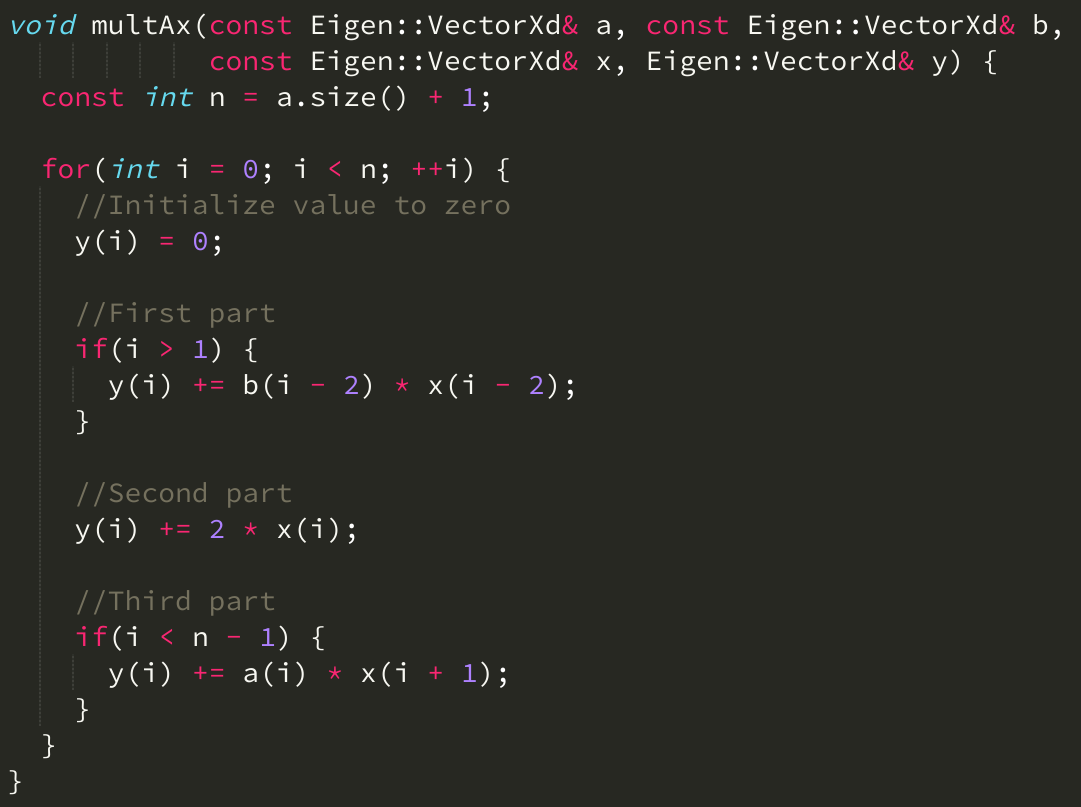
\includegraphics[width=1.0\linewidth]{2-6.a.png}
\end{figure}

\subsection*{2-6.b}
We are now tasked with showing that $\mathbf{A}$ is invertible if $a_{i}, b_{i} \in \left[0,1\right]$. Using the hint we can see that the condition $a_{i}, b_{i} \in \left[0,1\right]$ puts a restriction on the elements inside the kernel. Let us hence look at the equation $\mathbf{A}\mathbf{x} = \mathbf{0}$ for an example.
\begin{equation*}
    \begin{bmatrix}
    2 & a_{1} & 0 & 0 & 0 & 0& 0 \\
    0 & 2 & a_{2} & 0 & 0& 0 & 0 \\
    b_{1} & 0 & 2 & a_{3} & 0 & 0& 0 \\
    0 & b_{2} & 0& 2& a_{4} & 0& 0\\
    0 & 0 &b_{3} & 0 & 2 & a_{5} & 0\\
    0 & 0 & 0 & b_{4} & 0 & 2 & a_{6} \\
    0  & 0 & 0 & 0 & b_{5} & 0 & 2
    \end{bmatrix}
    \begin{bmatrix}
        x_{1} \\ x_{2} \\ x_{3} \\ x_{4} \\ x_{5} \\ x_{6} \\ x_{7}
    \end{bmatrix} =
    \begin{bmatrix}
        2x_{1} + a_{1}x_{2} \\
        2x_{2} + a_{2}x_{3} \\
        b_{1}x_{1} + 2x_{3} + a_{3}x_{4} \\
        b_{2}x_{2} + 2x_{4} + a_{4}x_{5} \\
        b_{3}x_{3} + 2x_{5} + a_{5}x_{6} \\
        b_{4}x_{4} + 2x_{6} + a_{6}x_{7} \\
        b_{5}x_{5} + 2x_{7}
    \end{bmatrix} = \begin{bmatrix}
        0 \\ 0  \\ 0 \\ 0 \\ 0 \\ 0 \\ 0
    \end{bmatrix}
\end{equation*}
We hence get the following system of equations to solve in general.
\begin{equation*}
    \begin{cases}
        0 &= 2x_{1} + a_{1}x_{2}  \\
        0&=2x_{2} + a_{2}x_{3}  \\
        0&=b_{1}x_{1} + 2x_{3} + a_{3}x_{4} \\
        0&=b_{2}x_{2} + 2x_{4} + a_{4}x_{5} \\
        \vdots&\phantom{=} \qquad \vdots \\
        0&=b_{n-3}x_{n-3} + 2x_{n-1} + a_{n-1}x_{n} \\
        0&=b_{n-2}x_{n-2} + 2x_{n}
    \end{cases}
\end{equation*}
The hint also tells us that we should conduct a proof by contradiction by assuming that the kernel is non-trivial $\text{ker} \: \mathbf{A} \neq \left\{0\right\}$ and then look at a solution $\mathbf{x} \in \text{ker} \: \mathbf{A}$ and consider its component with the largest absolute value (its modulus). Let $i = \text{argmax}\left\lvert x_{i}\right\rvert$ with $x_{i} \neq 0$, which is possible, as we have a solution which is non-trivial per assumption. We know must treat the cases separately for which $i = 1$, $i = 2$ or $i = n$, as the below argument does not work for these. We first make the proof for $x = 1$ (analogous for $x=2$). If $x = 1$ then we have ($x_{1} \neq 0$, because $x_{1}$ has the largest absolute value and $\mathbf{x}\neq 0$ by assumption)
\begin{equation*}
    0 = 2x_{1} + a_{1}x_{2} \implies 2x_{1} = -a_{1}x_{2} \implies 2 = -\left(\frac{x_{2}}{x_{1}}a_{1} \right) \implies \frac{x_{2}}{x_{1}}a_{1} = -2
\end{equation*}
From this we follow that 
\begin{equation*}
    \left\lvert \frac{x_{2}}{x_{1}}a_{1}\right\rvert = 2 \implies \left\lvert \frac{x_{2}}{x_{1}}\right\rvert \left\lvert a_{1}\right\rvert = 2 \implies  \frac{\left\lvert x_{2}\right\rvert}{\left\lvert x_{1}\right\rvert} \left\lvert a_{1}\right\rvert = 2 
\end{equation*}
Because $x_{1}$ has the greatest absolute value of all components we can at most have $\left\lvert x_{1}\right\rvert = \left\lvert x_{2}\right\rvert$ and hence we must have $\left\lvert a_{1}\right\rvert \geq 2$ for this to be satisfied, which is a contradiction to the assumption that $a_{i} \in \left[0,1\right]$ for all $i$. The other special case is when the $x_{i}$ with the largest absolute value is $x_{n}$ and thus $0 = b_{n-2}x_{n-2} + 2x_{n}$  gives us (again remember that $x_{n} \neq 0$)
\begin{equation*}
   0 = b_{n-2}x_{n-2} + 2x_{n}\implies 2x_{n} = -b_{n-2}x_{n-2} \implies  2 = -\left(\frac{x_{n-2}}{x_{n}}b_{n-2}\right) \implies \left(\frac{x_{n-2}}{x_{n}}b_{n-2}\right) = -2
\end{equation*}
from which we follow
\begin{equation*}
    \left\lvert\frac{x_{n-2}}{x_{n}}b_{n-2}\right\rvert = 2 \implies \left\lvert \frac{x_{n-2}}{x_{n}}\right\rvert \left\lvert b_{n-2}\right\rvert = 2 \implies  \frac{\left\lvert x_{n-2}\right\rvert}{\left\lvert x_{n}\right\rvert} \left\lvert b_{n-2}\right\rvert = 2 
\end{equation*}
With the same argument as above we follow that $\left\lvert b_{n-2}\right\rvert \geq 2$ must be true, which again is a contradiction to the assumption that $a_{i}, b_{i} \in \left[0,1\right]$ for all $i$.

\pagebreak 

\noindent In the general case ($x_{i}, 2 > i > n$ is the component with the greatest absolute value) we then have 
\begin{equation*}
    b_{i-2}x_{i-2} + 2x_{i} + a_{i}x_{i+1} = 0 \implies \frac{1}{x_{i}}\left(-a_{i}x_{i+1} - b_{i-2}x_{i-2}\right) = 2
\end{equation*}
We are allowed to do the last step because we said that $x_{i} \neq 0$. This then gives us
\begin{align*}
    -\left(\frac{x_{i+1}}{x_{i}}a_{i} + \frac{x_{i-2}}{x_{i}}b_{i-2}\right) = 2 &\implies \frac{x_{i+1}}{x_{i}}a_{i} + \frac{x_{i-2}}{x_{i}}b_{i-2} = -2 \\
    &\implies \left\lvert \frac{x_{i+1}}{x_{i}}a_{i} + \frac{x_{i-2}}{x_{i}}b_{i-2}\right\rvert =2
\end{align*}
We then have 
\begin{align*}
    \left\lvert \frac{x_{i+1}}{x_{i}}a_{i} + \frac{x_{i-2}}{x_{i}}b_{i-2}\right\rvert \overset{\Delta\text{-ineq.}}{\leq} \left\lvert \frac{x_{i+1}}{x_{i}}a_{i}\right\rvert  + \left\lvert \frac{x_{i-2}}{x_{i}}b_{i-2}\right\rvert  &\leq \frac{\left\lvert x_{i+1}\right\rvert }{\left\lvert x_{i}\right\rvert }\left\lvert a_{i}\right\rvert  + \frac{\left\lvert x_{i-2} \right\rvert }{\left\lvert x_{i}\right\rvert }\left\lvert b_{i-2}\right\rvert  \\[2mm]
    &\leq 1\left\lvert a_{i}\right\rvert  + 1\left\lvert b_{i-2}\right\rvert \\
    &= \left\lvert a_{i}\right\rvert  + \left\lvert b_{i-2}\right\rvert \\
    &= 1 + 1 \\ 
    &= 2
\end{align*}
We have used $\left\lvert x_{i} \right\rvert = \left\lvert x_{i+1} \right\rvert$ and $\left\lvert x_{i} \right\rvert = \left\lvert x_{i-2} \right\rvert$ in one of the steps and $\left\lvert a_{i}\right\rvert = 1$ and $\left\lvert b_{i-2}\right\rvert = 1$ in another step and only under these assumptions is it even possible for the equations $3$ to $n-1$ to hold. We must have that $\left\lvert x_{i}\right\rvert = \left\lvert x_{j}\right\rvert $ for all $2 < i < j < n$ as a consequence. Putting this into one of the equations would then give us
\begin{equation}
    b_{i-2}x_{i-2} + 2x_{i} + a_{i}x_{i+1} = 0
\end{equation}
We know have multiple ways $x_{i}$, $x_{i+1}$ and $x_{i-2}$ could depend on each other. Let us list up some of them
\begin{align*}
    x_{i} &= \phantom{-}x_{i +1} = \phantom{-}x_{i-2} \\
    x_{i} &= -x_{i +1} = \phantom{-}x_{i-2} \\
    x_{i} &= -x_{i +1} = -x_{i-2} \\
\end{align*}
Let us consider these three cases and make a general statement about all that exist. In the first case we get (keep in mind that because $x_{i} \neq 0$ now all $x_{j} \neq 0$ in this case)
\begin{equation*}
    b_{i-2}x_{i-2} + 2x_{i} + a_{i}x_{i+1} = 0\Longleftrightarrow x_{i}\left(b_{i-2} + 2 + a_{i}\right) = 0\Longleftrightarrow b_{i-2} + 2 + a_{i} = 0 
\end{equation*}
This equation cannot be satisfied as $a_{i}, b_{i-2} \in \left[0,1\right]$. We then have (in the second case)
\begin{equation*}
   b_{i-2}x_{i-2} + 2x_{i} + a_{i}x_{i+1} = 0\Longleftrightarrow x_{i}\left(b_{i-2} + 2 - a_{i}\right) = 0\Longleftrightarrow b_{i-2} + 2 - a_{i} = 0  
\end{equation*}
This can again not be satisfied for the same reason as above. The third case is more interesting though. 
\begin{equation*}
    b_{i-2}x_{i-2} + 2x_{i} + a_{i}x_{i+1} = 0\Longleftrightarrow x_{i}\left(-b_{i-2} + 2 - a_{i}\right) = 0\Longleftrightarrow -b_{i-2} + 2 - a_{i} = 0 
\end{equation*}
This case is possible and is the only case which is possible overall. All others will lead to an unsatisfiable equation. For this to be satisfied we would need $a_{i} = b_{i-2} = 1$ for all $2 < i < n$. What can we do now? We argue that because all components have the same absolute value $x_{1}$, $x_{2}$ and $x_{n}$ also have the greatest absolute value and thus we can just use the contradictions we produced in these cases for this case as well. This concludes the proof as in all cases we produced a contradition meaning that the assumption was false and thus $\text{ker}\:\mathbf{A} = \left\{0\right\}$ follows as a consequence. Hence we can conclude that if $a_{i}, b_{i} \in \left[0,1\right]$ for all $i$, then $\mathbf{A}$ is regular and hence invertible.
\subsection*{2-6.c}
We can now assume that $b_{i} = 0$ for all $i = 1,\dots, n-2$ and are tasked with implementing an efficient \verb|C++| function solving the LSE $\mathbf{A}\mathbf{x} = \mathbf{r}$. We first observe the structure.
\begin{equation*}
    \begin{bmatrix}
    2 & a_{1} & 0 & 0 & 0 & 0& 0 \\
    0 & 2 & a_{2} & 0 & 0& 0 & 0 \\
    0 & 0 & 2 & a_{3} & 0 & 0& 0 \\
    0 & 0 & 0& 2& a_{4} & 0& 0\\
    0 & 0 &0 & 0 & 2 & a_{5} & 0\\
    0 & 0 & 0 & 0 & 0 & 2 & a_{6} \\
    0  & 0 & 0 & 0 & 0 & 0 & 2
    \end{bmatrix}
    \begin{bmatrix}
        x_{1} \\ x_{2} \\ x_{3} \\ x_{4} \\ x_{5} \\ x_{6} \\ x_{7}
    \end{bmatrix} =
    \begin{bmatrix}
        2x_{1} + a_{1}x_{2} \\
        2x_{2} + a_{2}x_{3} \\
        2x_{3} + a_{3}x_{4} \\
        2x_{4} + a_{4}x_{5} \\
        2x_{5} + a_{5}x_{6} \\
        2x_{6} + a_{6}x_{7} \\
        2x_{7}
    \end{bmatrix} = \begin{bmatrix}
        r_{1} \\ r_{2}  \\ r_{3} \\ r_{4} \\ r_{5} \\ r_{6} \\ r_{7}
    \end{bmatrix}
\end{equation*}
We can see that we can solve this system by starting at the bottom with $x_{7} = \frac{r_{7}}{2}$ and then for each next equation we have
\begin{equation*}
    2x_{i} + a_{i}x_{i+1} = r_{i} \implies 2x_{i} = r_{i} - a_{i}x_{i+1} \implies x_{i} = \frac{1}{2}\left(r_{i} - a_{i}x_{i+1}\right)
\end{equation*}
This produces the following code.
\begin{figure}[!hbt]
    \centering
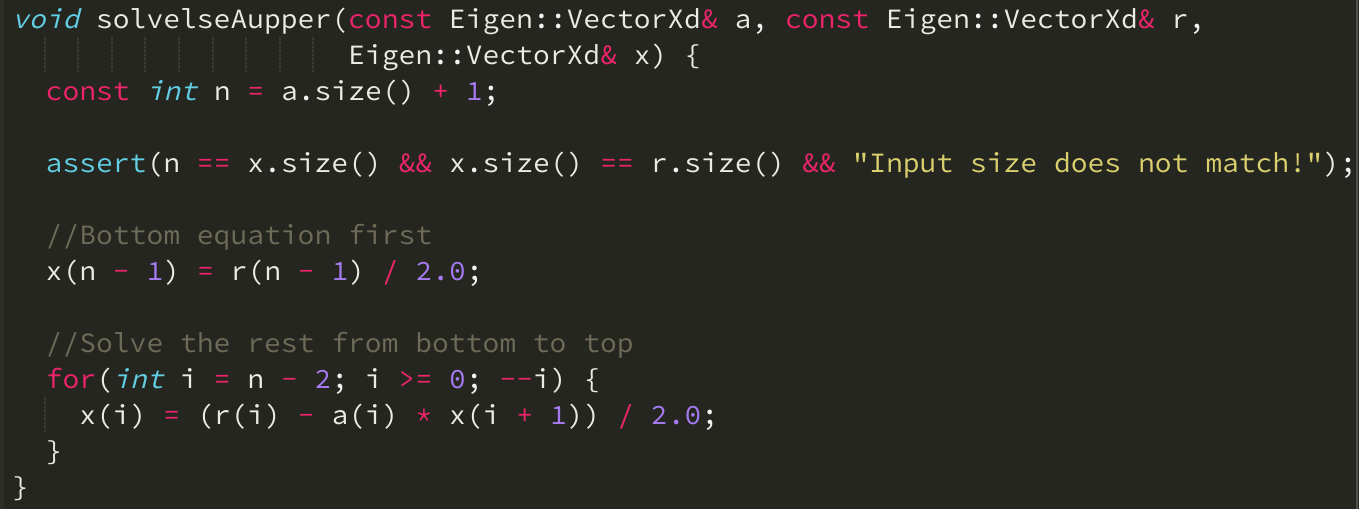
\includegraphics[width=0.9\linewidth]{2-6.c.png}
\end{figure}

\subsection*{2.6-d}
We are now tasked to solve the LSE $\mathbf{A}\mathbf{x} = \mathbf{r}$ for general $a_{i}, b_{i} \in \left[0,1\right]$ in an efficient way. We again consider the given structure using an example.
\begin{equation*}
    \begin{bmatrix}
    2 & a_{1} & 0 & 0 & 0 & 0& 0 \\
    0 & 2 & a_{2} & 0 & 0& 0 & 0 \\
    b_{1} & 0 & 2 & a_{3} & 0 & 0& 0 \\
    0 & b_{2} & 0& 2& a_{4} & 0& 0\\
    0 & 0 &b_{3} & 0 & 2 & a_{5} & 0\\
    0 & 0 & 0 & b_{4} & 0 & 2 & a_{6} \\
    0  & 0 & 0 & 0 & b_{5} & 0 & 2
    \end{bmatrix}
    \begin{bmatrix}
        x_{1} \\ x_{2} \\ x_{3} \\ x_{4} \\ x_{5} \\ x_{6} \\ x_{7}
    \end{bmatrix} =
    \begin{bmatrix}
        2x_{1} + a_{1}x_{2} \\
        2x_{2} + a_{2}x_{3} \\
        b_{1}x_{1} + 2x_{3} + a_{3}x_{4} \\
        b_{2}x_{2} + 2x_{4} + a_{4}x_{5} \\
        b_{3}x_{3} + 2x_{5} + a_{5}x_{6} \\
        b_{4}x_{4} + 2x_{6} + a_{6}x_{7} \\
        b_{5}x_{5} + 2x_{7}
    \end{bmatrix} = \begin{bmatrix}
        r_{1} \\ r_{2}  \\ r_{3} \\ r_{4} \\ r_{5} \\ r_{6} \\ r_{7}
    \end{bmatrix}
\end{equation*}
This structure does not allow us to solve it directly as in 2-6.c. We must apply Gaussian elimination here. We do rely on the renaming technique introduced in the solution to make our work a bit more pleasant.

\begin{align*}
    \begin{vmatrix}
    2 & a_{1} & 0 & 0   \\
    0 & 2 & a_{2} & 0   \\
    b_{1} & 0 & 2 & a_{3}  \\
    0 & b_{2} & 0& 2\\
    \end{vmatrix}
    \begin{vmatrix}
        r_{1} \\ r_{2}  \\ r_{3} \\ r_{4}
    \end{vmatrix} &\longrightarrow 
    \begin{vmatrix}
    2 & a_{1} & 0 & 0  \\
    0 & 2 & a_{2} & 0  \\
    b_{1} - b_{1} & 0 - \frac{b_{1}}{2}a_{1} & 2 & a_{3} \\
    0 & b_{2} & 0& 2\\
    \end{vmatrix}
    \begin{vmatrix}
        r_{1} \\ r_{2}  \\ r_{3} - \frac{b_{1}}{2}r_{1} \\ r_{4}
    \end{vmatrix}   \\[1mm]
    &\longrightarrow 
    \begin{vmatrix}
    2 & a_{1} & 0 & 0  \\
    0 & 2 & a_{2} & 0  \\
    0 & c_{2} & 2 & a_{3} \\
    0 & b_{2} & 0& 2\\
    \end{vmatrix}
    \begin{vmatrix}
        r_{1} \\ r_{2}  \\ r_{3} - \frac{b_{1}}{2}r_{1} \\ r_{4}
    \end{vmatrix} \\[1mm]
    &\longrightarrow 
    \begin{vmatrix}
    2 & a_{1} & 0 & 0  \\
    0 & 2 & a_{2} & 0  \\
    0 & c_{2} -c_{2} & 2-\frac{c_{2}}{2}a_{2} & a_{3}\\
    0 & b_{2}-b_{2} & 0 - \frac{b_{2}}{2}a_{2}& 2\\
    \end{vmatrix}
    \begin{vmatrix}
        r_{1} \\ r_{2}  \\ r_{3} - \frac{b_{1}}{2}r_{1} -\frac{c_{2}}{2}r_{2} \\ r_{4} - \frac{b_{2}}{2}r_{3}
    \end{vmatrix}  \\[1mm]
    &\longrightarrow 
    \begin{vmatrix}
    2 & a_{1} & 0 & 0  \\
    0 & 2 & a_{2} & 0  \\
    0 & 0 & d_{3}& a_{3}\\
    0 & 0& c_{3}& 2\\
    \end{vmatrix}
    \begin{vmatrix}
        r_{1} \\ r_{2}  \\ r_{3} - \frac{b_{1}}{2}r_{1} -\frac{c_{2}}{2}r_{2}  \\ r_{4} - \frac{b_{2}}{2}r_{3}
    \end{vmatrix} \\[1mm]
    &\longrightarrow 
    \begin{vmatrix}
    2 & a_{1} & 0 & 0  \\
    0 & 2 & a_{2} & 0  \\
    0 & 0 & d_{3}& a_{3}\\
    0 & 0& c_{3} - c_{3}& 2 - \frac{c_{3}}{d_{3}}a_{3}\\
    \end{vmatrix}
    \begin{vmatrix}
        r_{1} \\ r_{2}  \\ r_{3} - \frac{b_{1}}{2}r_{1} -\frac{c_{2}}{2}r_{2}  \\ r_{4} - \frac{b_{2}}{2}r_{3} - \frac{c_{3}}{d_{3}}r'_{3}
    \end{vmatrix}  \\[1mm]
    &\longrightarrow 
    \begin{vmatrix}
    2 & a_{1} & 0 & 0  \\
    0 & 2 & a_{2} & 0  \\
    0 & 0 & d_{3}& a_{3}\\
    0 & 0& 0& d_{4}
    \end{vmatrix}
    \begin{vmatrix}
        r_{1} \\ r_{2}  \\ r_{3} - \frac{b_{1}}{2}r_{1} -\frac{c_{2}}{2}r_{2} \\ r_{4} - \frac{b_{2}}{2}r_{3} - \frac{c_{3}}{d_{3}}r'_{3}
    \end{vmatrix} 
\end{align*}

\pagebreak

 \noindent We can see that we get a recurring pattern given by the following recurrence relation ($c_{1}=0$, $d_{1} = d_{2} = 2$), one must use a bigger matrix to truly see how the recurrence relation for $d_{i+1}$ is derived.
 \begin{align*}
     c_{i+1} &= -\frac{b_{i}}{c_{i}}a_{i} \\
     d_{i+1} &= d_{i + 1} - \frac{c_{i}}{d_{i}}a_{i} 
 \end{align*}
 We then have the recurrence relations for $r_{i}$, seeing as $d_{2} = 2$, we get in each step two terms that we deduct from the current $r_{i}$, which gives us
 \begin{equation*}
     r_{i+1} = r_{i+1} - \frac{b_{i -1}}{d_{i - 1}}r_{i - 1}- \frac{c_{i}}{d_{i}}r_{i}  \: \text{(only correct at the start -\> two step process)}
 \end{equation*}
We will have to ensure that we use  the correct value for $r_{i}'$, hence in the code we will split this process into two parts, as in each step both $r_{i+1}$ and $r_{i+2}$ are updated. We can then use backwards substitution to solve the system, in each step we still need the old value of $r_{i}$, so we must store this separately. In the code we use the result vector \verb|x| for this purpose, then we do not have to add it to the result later on. This results in the following code.
\begin{figure}[!hbt]
    \centering
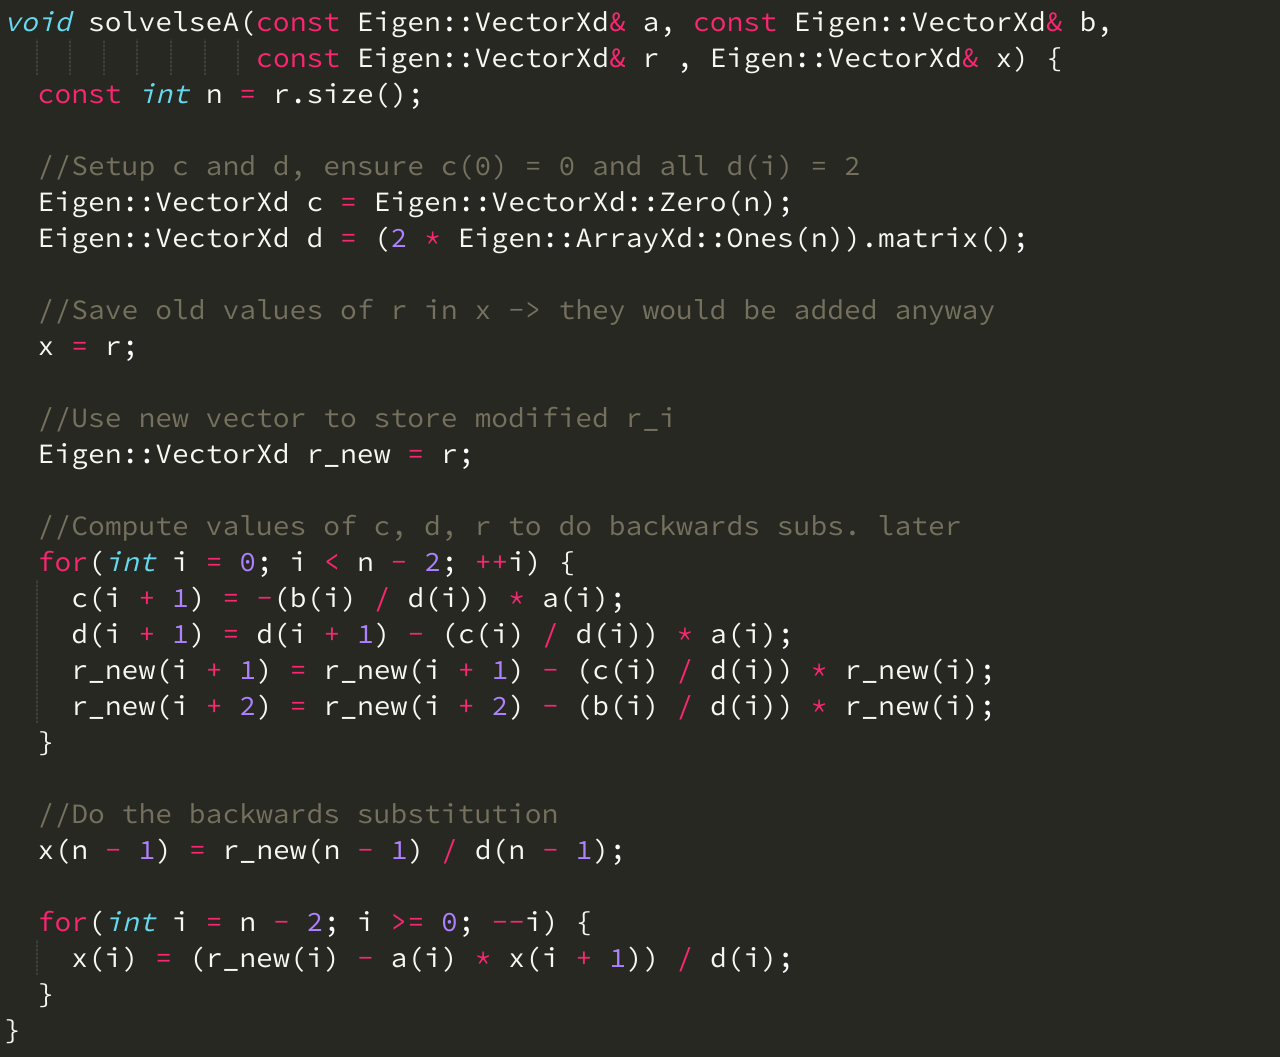
\includegraphics[width=1.0\linewidth]{2-6.d.png}
\end{figure}
I am unsure if the above formula could work if implemented correctly, but this two step process is more elegant and works well.

\pagebreak

\subsection*{2.6-e} 
We are now tasked with determining the asymptotic complexity of our implementation of \verb|solvelseA|. Creating and copying arrays can be done in $\mathcal{O}\left(n\right)$, the first loop takes also $\mathcal{O}\left(n\right)$, as all computations inside of the loop only take a constant amount of time, the second loop also requires$\mathcal{O}\left(n\right)$ time, for the same reason. Overall we thus get $\mathcal{O}\left(n\right)$. 

\subsection*{2-6.f} 
We should now implement the same LSE solver as in 2-6.d, but now use the sparse matrix solving utilities of Eigen. We must first remember some important functionality of Eigen. We will use an example from the lecture document for this purpose, which is given on page 178  in chapter 2.7.3.

\begin{figure}[!hbt]
    \centering
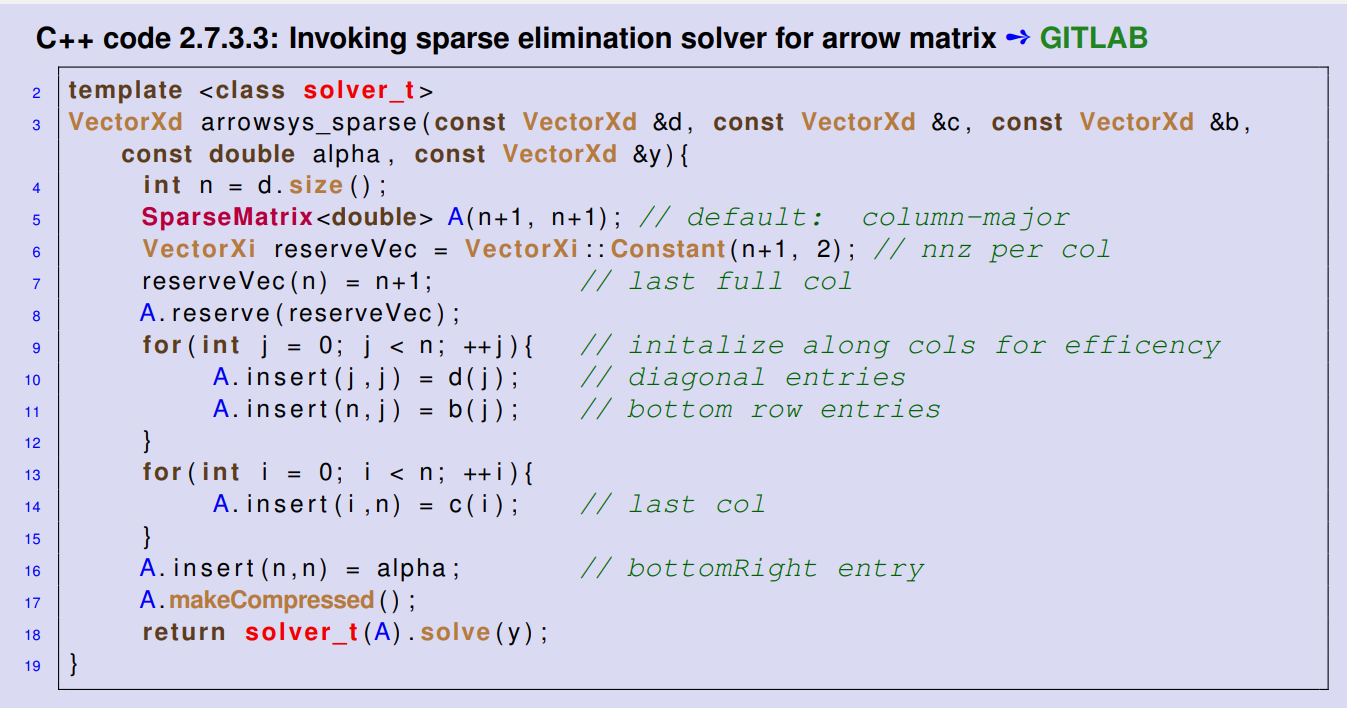
\includegraphics[width=0.8\linewidth]{SparseMatricesEigen.png}
\end{figure}
\noindent This gives us the following code.

\begin{figure}[!hbt]
    \centering
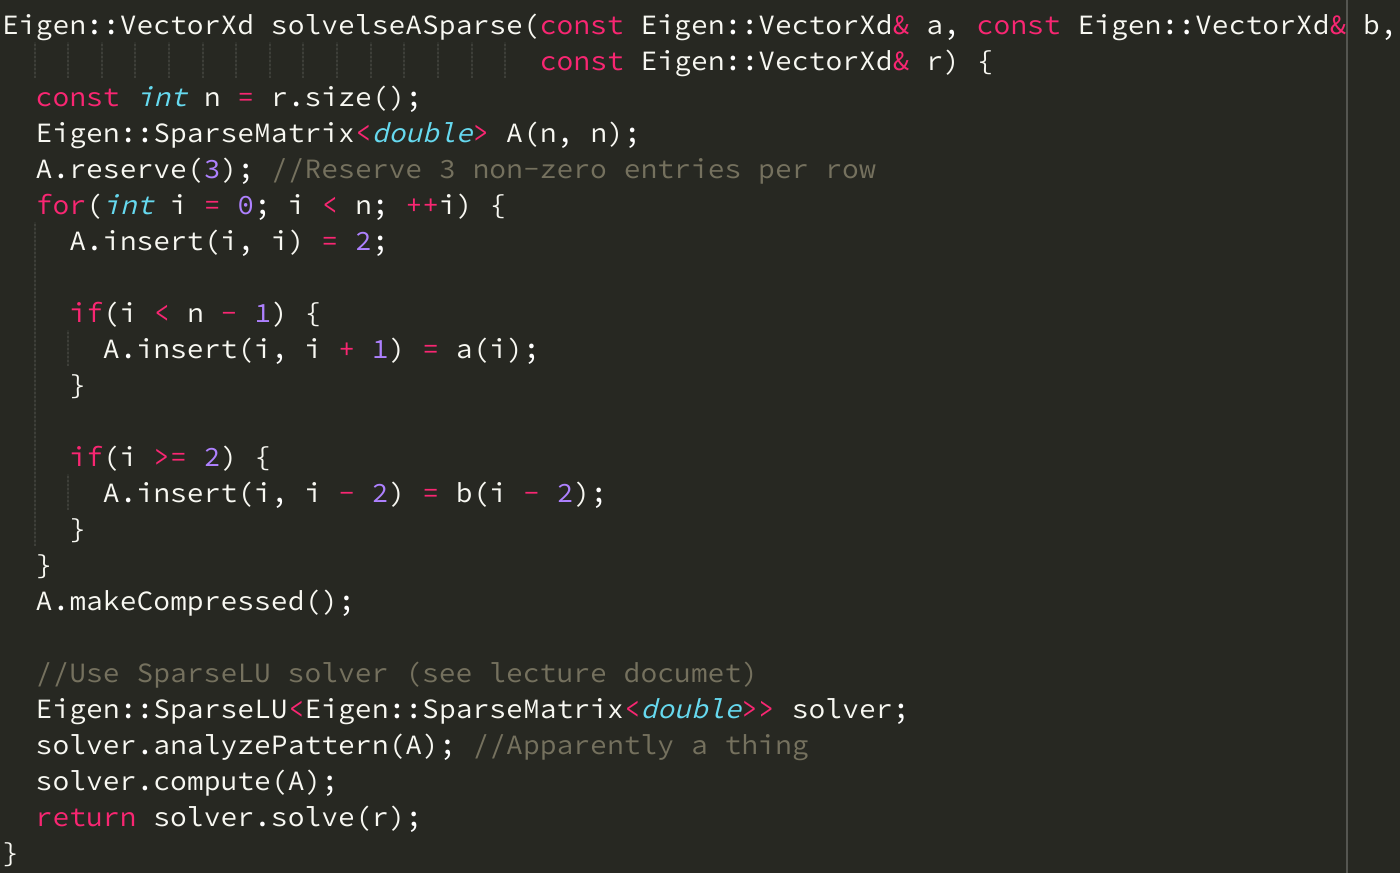
\includegraphics[width=0.8\linewidth]{2-6.f.png}
\end{figure}
Remember to include \verb|<Eigen/Sparse>|

\end{document}
